% =====================================================================
\chapter{Du papier au code avec Claude Code}
\label{ch:18}
% =====================================================================

\section{Objectifs et organisation du chapitre}

\paragraph{Objectifs.} Ce dernier chapitre transforme le cours en méthode de production. À la fin, vous saurez : (1) rédiger un cahier des charges qu'un assistant de programmation peut transformer en code vérifiable ; (2) organiser le paquet \texttt{arbhub} et ses tests ; (3) garantir que le code exécuté en \emph{paper trading} est exactement celui qui a été testé (\og parité\fg) ; (4) appliquer une grille de critères de passage chiffrés avant d'engager de l'argent ; (5) mesurer l'effet du retard d'exécution ; (6) surveiller une stratégie en \emph{paper trading} sans multiplier les fausses alarmes ; (7) déployer progressivement et tenir un journal.

\paragraph{Code.}\sloppy \texttt{code/ch18/ch18\_pipeline.py} (E1 à E4) ; modules \texttt{src/arbhub/signals/pair\_strategy.py} et \texttt{src/arbhub/data/loaders.py}, tests \texttt{tests/test\_pair\_strategy.py} ; modèle de cahier des charges \texttt{docs/specs/TEMPLATE\_strategie.md} ; intégration continue \texttt{.github/workflows/tests.yml}.

\begin{intuition}
Un pilote ne décolle pas parce qu'il \og sent\fg{} que l'avion est prêt : il déroule une liste de contrôle écrite à l'avance, et un seul point rouge suffit à rester au sol. Ce chapitre construit la liste de contrôle d'une stratégie : le cahier des charges est le plan de vol, les tests sont les vérifications techniques, les critères de passage sont la liste avant décollage, et le \emph{paper trading} est le vol d'essai.
\end{intuition}

% =====================================================================
\section{Le cycle de développement}
% =====================================================================

\begin{enumerate}
\item \textbf{Cahier des charges} (\texttt{docs/specs/}) : hypothèse économique, données, modèle, règles, coûts déclarés, variantes prévues, critères de passage, tests exigés, plan de déploiement. Rédigé \emph{avant} tout code.
\item \textbf{Tests d'abord} : les propriétés exigées (absence d'anticipation, parité, coûts, limites) sont écrites comme tests qui échouent \citep{beck2002}.
\item \textbf{Implémentation} dans \texttt{src/arbhub/}, jusqu'à ce que les tests passent.
\item \textbf{Recherche} dans \texttt{code/} : \emph{backtest} hors échantillon, nombre de variantes consigné.
\item \textbf{Critères de passage} : décision écrite \og go\fg{} ou \og no-go\fg.
\item \textbf{\emph{Paper trading}} avec contrôles datés à l'avance.
\item \textbf{Petite taille réelle}, puis \textbf{taille cible}.
\item \textbf{Revue mensuelle} : réel contre \emph{backtest}, incidents, décisions.
\end{enumerate}

\subsection{Travailler avec Claude Code}

Un assistant de programmation est très efficace pour écrire du code, et tout aussi efficace pour écrire du code faux qui \og a l'air juste\fg. Trois règles en tirent le meilleur parti.

\begin{description}
\item[Spécifier des propriétés, pas seulement des fonctions.] \og Écris une fonction de \emph{z-score}\fg{} produit une fonction. \og Écris une fonction de \emph{z-score} et un test qui vérifie que modifier les données après $t$ ne change pas $z_t$\fg{} produit une fonction \emph{vérifiée}.
\item[Fixer les règles une fois pour toutes.] Le fichier \texttt{CLAUDE.md} à la racine du dépôt est lu automatiquement par Claude Code. Il contient les règles du cours : aucune anticipation, formation et test séparés, coûts explicites, nombre de variantes consigné, aucun ordre réel sans validation humaine, pas de stratégie inter-plateformes sur un compte de \emph{prop firm}.
\item[Relire ce qui compte.] Le code d'exécution et de risque (ce qui envoie des ordres) se relit ligne par ligne, quelle que soit sa provenance. Le dépôt \texttt{atjte} rappelle lui-même qu'il a été écrit en grande partie avec des assistants et n'a pas été audité \citep{atjte}.
\end{description}

\begin{whiteboard}[ — modèle de demande à Claude Code]
\small\og Lis \texttt{docs/specs/paire\_XXX.md}. Écris d'abord dans \texttt{tests/} : (a) un test d'absence d'anticipation, (b) un test de parité entre la version vectorisée et \texttt{on\_bar}, (c) un test des coûts. Puis implémente dans \texttt{src/arbhub/signals/} jusqu'à ce que \texttt{pytest} passe. Ensuite, écris \texttt{code/strategies/paire\_XXX.py} qui applique les critères de passage du chapitre 18 avec les $N$ variantes listées dans la spécification, et enregistre les résultats en JSON. Ne modifie aucun test existant.\fg
\end{whiteboard}

% =====================================================================
\section{Architecture du paquet \texttt{arbhub}}
% =====================================================================

\begin{center}\small
\begin{tabularx}{\textwidth}{>{\footnotesize\ttfamily}p{4.5cm}>{\raggedright}X>{\raggedright\arraybackslash}p{1.6cm}}
\toprule
\normalfont Module & Contenu & Chapitres \\
\midrule
data/loaders.py & Seul module qui lit le disque ; contrôles de validité des prix. & 3, 18 \\
stats/mean\_reversion.py & AR(1), demi-vie, \emph{z-score} de formation. & 1, 5 \\
signals/pair\_strategy.py & Stratégie de paire : version vectorisée et version événementielle. & 7, 18 \\
backtest/engine.py & Moteur sans anticipation, coûts par jambe. & 16 \\
backtest/metrics.py & Sharpe, erreur-type, PSR, DSR, PBO, drawdown. & 16 \\
risk/sizing.py & Kelly, ciblage de volatilité, CUSUM, $\hat\varphi$ glissant. & 17 \\
models/, execution/ & À compléter : Kalman, copules, OU ; simulateur d'exécution, connecteurs. & 5, 8, 9, 15 \\
\bottomrule
\end{tabularx}
\end{center}

Principes : fonctions pures autant que possible (mêmes entrées, mêmes sorties, aucun effet de bord) ; entrées et sorties isolées dans \texttt{data/} et, plus tard, \texttt{execution/} ; chaque fonction a au moins un test ; l'intégration continue (GitHub Actions) relance tous les tests à chaque envoi sur le dépôt. La suite compte 24 tests à la fin de ce chapitre.

% =====================================================================
\section{La parité recherche / production}
% =====================================================================

Un \emph{backtest} vectorisé calcule toutes les positions d'un coup ; un robot reçoit les prix un par un. Ce sont deux programmes différents, et rien ne garantit qu'ils prennent les mêmes décisions : un indice décalé, une fenêtre qui inclut ou non la séance courante, un état mal réinitialisé suffisent. Si les deux divergent, le \emph{backtest} ne dit rien du robot.

Le module \texttt{pair\_strategy} fournit les deux versions de la même stratégie : écart en log-prix $\ln y_t - \hat\alpha_t - \hat\beta_t\ln x_t$ avec $(\hat\alpha_t,\hat\beta_t)$ estimés par moindres carrés sur une fenêtre glissante, \emph{z-score} glissant, règle à hystérésis avec stop. La configuration est validée à la construction (fenêtre du \emph{z-score} plus courte que celle de la régression, $0 \le$ sortie $<$ entrée $<$ stop).

\begin{lstlisting}[language=Python]
from arbhub.signals.pair_strategy import PairConfig, PairStrategy, vectorized_positions
cfg = PairConfig(beta_window=120, z_window=60, entry=2.0, exit=0.0, stop=4.0)
q, beta, z = vectorized_positions(y, x, cfg)          # recherche
bot = PairStrategy(cfg)
for y_close, x_close in flux_de_clotures():           # production
    target, beta_t, z_t = bot.on_bar(y_close, x_close)
\end{lstlisting}

\begin{codebox}[ — E1, parité sur données réelles (500 séances)]
Version événementielle contre version vectorisée, configuration ci-dessus. \textbf{KO/PEP :} écart maximal des positions $0$, écart maximal des $\hat\beta_t$ $0$, 16 changements de position. \textbf{GLD/GLDM :} écarts nuls, 20 changements de position. Le test \texttt{test\_event\_driven\_matches\_vectorized} vérifie la même égalité à chaque modification du code.
\end{codebox}

% =====================================================================
\section{Les critères de passage}
% =====================================================================

\subsection{La grille}

Une stratégie ne passe au \emph{paper trading} que si elle satisfait \emph{tous} les critères suivants, calculés sans jamais regarder la période de test pour choisir quoi que ce soit.

\begin{center}\small
\begin{tabularx}{\textwidth}{>{\bfseries}p{0.7cm}>{\raggedright}p{4.6cm}>{\raggedright\arraybackslash}X}
\toprule
\normalfont & Critère & Justification \\
\midrule
G0 & Hypothèse économique écrite & Sans ancre, une relation statistique est suspecte (chapitres~0 et~7). \\
G1 & Engle-Granger $p<0{,}05$ sur la formation & Écart stationnaire (chapitres~3 et~4). \\
G2 & Demi-vie entre 1 et 30 séances & Observable à la fréquence choisie et assez rapide pour le capital (chapitres~1 et~5). \\
G3 & DSR $>0{,}95$ avec toutes les variantes essayées & Le meilleur réglage bat le hasard de la sélection (chapitre~16). \\
G4 & Gain net positif sur le test & Le résultat survit hors échantillon. \\
G5 & Coût de rentabilité nulle $> 2\times$ coût déclaré & Marge de sécurité sur les frictions (chapitres~12 et~16). \\
\bottomrule
\end{tabularx}
\end{center}

\subsection{Application à trois candidats}

\begin{codebox}[ — E2, critères de passage (formation : 250 séances ; test : 250 séances ; 12 variantes ; 5 pb par jambe)]
\begin{center}\small
\begin{tabular}{lccccc}
\toprule
 & Simulée 1 & Simulée 2 & Simulée 3 & KO/PEP & GLD/GLDM \\
\midrule
$p$ Engle-Granger & 0,0001 & 0,0019 & 0,048 & 0,097 & $<0{,}0001$ \\
Demi-vie (séances) & 3,2 & 4,8 & 3,4 & 10,6 & 0,4 \\
Sharpe formation (meilleure variante) & 4,37 & 2,33 & 3,51 & 2,12 & $-1{,}48$ \\
DSR & 1,000 & 0,814 & 0,951 & 0,356 & 0,002 \\
Sharpe test net & 2,61 & 2,60 & 2,10 & 0,19 & $-1{,}60$ \\
Rendement test net & 12,9\,\% & 16,0\,\% & 16,1\,\% & 3,1\,\% & $-0{,}7\,\%$ \\
Coût de rentabilité nulle (pb) & 51,3 & 44,0 & 26,9 & 19,7 & 2,2 \\
\midrule
Critères échoués & aucun & G3 & aucun & G1, G3 & G2 à G5 \\
Décision & \textbf{go} & no-go & \textbf{go} & no-go & no-go \\
\bottomrule
\end{tabular}
\end{center}
Les trois paires simulées sont réellement cointégrées (demi-vie vraie de 4,3 séances).
\end{codebox}

\begin{figure}[h]
\centering
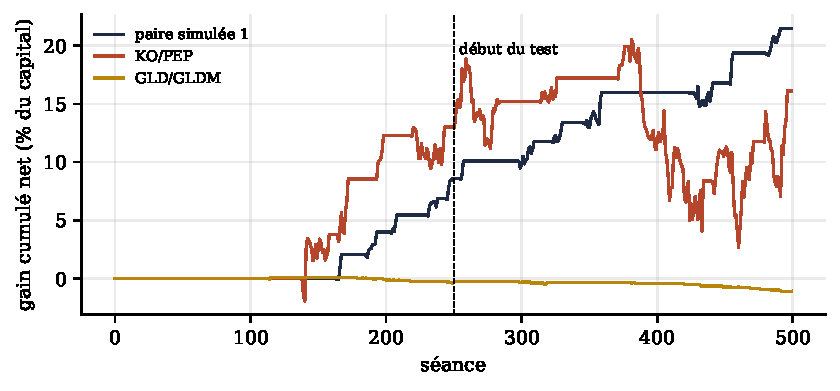
\includegraphics[width=0.85\textwidth]{ch18/go_nogo.pdf}
\caption{Gain cumulé net de la variante retenue sur la formation pour trois candidats ; la ligne pointillée sépare formation et test.}
\label{c18:fig:gonogo}
\end{figure}

\paragraph{Lecture.}
\begin{enumerate}
\item \textbf{KO/PEP} est l'exemple le plus instructif : la meilleure des 12 variantes affiche un Sharpe de 2,1 sur la formation et un gain positif sur le test (3,1\,\%). Un trader pressé déploierait. La grille dit non : la paire n'est pas cointégrée au seuil de 5\,\% et, une fois compté le nombre de variantes, le Sharpe de formation n'est pas distinguable du hasard (DSR $0{,}36$). Le Sharpe du test ($0{,}19$) le confirme a posteriori.
\item \textbf{GLD/GLDM} est parfaitement cointégrée, mais son écart revient en moins d'une séance et vaut quelques points de base : à 5 pb par jambe, aucune règle quotidienne ne couvre ses coûts (rentabilité nulle à 2,2 pb). Une relation très solide n'est pas une stratégie rentable ; elle relève, au mieux, de l'exécution intrajournalière du chapitre~15.
\item \textbf{La paire simulée 2}, pourtant réellement cointégrée, échoue au DSR sur un an de formation. La grille est volontairement conservatrice : elle rejette parfois une bonne paire. C'est le prix d'éviter d'accepter les mauvaises ; une paire rejetée de peu peut être remise en observation (\emph{paper trading} sans engagement) plutôt qu'abandonnée.
\end{enumerate}

% =====================================================================
\section{Le retard d'exécution}
% =====================================================================

Un \emph{backtest} sur clôtures suppose qu'on est exécuté au prix de clôture qui a servi à décider. En pratique, on décide après la clôture et on est exécuté plus tard : à l'ouverture suivante, ou à la clôture suivante avec un ordre au marché de clôture.

\begin{codebox}[ — E3, décider à la clôture de $t$, être exécuté à la clôture de $t+1$ (200 mondes de 1\,000 séances, 5 pb)]
\begin{center}\small
\begin{tabular}{ccccc}
\toprule
$\varphi$ & Demi-vie & Sharpe, exécution & Sharpe, exécution & Perte \\
 & & à la clôture & le lendemain & \\
\midrule
0,50 & 1,0 & 3,20 & 1,47 & $-54\,\%$ \\
0,80 & 3,1 & 2,48 & 1,93 & $-22\,\%$ \\
0,90 & 6,6 & 1,76 & 1,57 & $-11\,\%$ \\
0,95 & 13,5 & 1,15 & 1,06 & $-8\,\%$ \\
\bottomrule
\end{tabular}
\end{center}
\end{codebox}

\paragraph{Lecture.} Plus l'écart revient vite, plus un jour de retard coûte cher : avec une demi-vie d'une séance, la moitié du Sharpe disparaît. Une stratégie à demi-vie courte n'est exploitable que si l'exécution est rapide (ordres au marché de clôture, ou données et exécution intrajournalières). Le \emph{backtest} doit modéliser le délai réel d'exécution, pas le délai idéal.

% =====================================================================
\section{Surveiller le \emph{paper trading}}
% =====================================================================

\subsection{La question}

Après quelques semaines de \emph{paper trading}, la stratégie fait moins bien que son \emph{backtest}. Malchance ou \emph{backtest} trop optimiste ? On teste l'hypothèse \og le vrai Sharpe est celui du \emph{backtest}\fg{} avec la statistique
\[
Z_T = \frac{\widehat{SR}_{\text{réel},T} - SR_{\text{backtest}}}{\sqrt{1/(T-1)}},
\]
qui suit approximativement une loi normale centrée réduite sous cette hypothèse (proposition~\ref{c16:prop:sese}). On conclut à la sous-performance si $Z_T < -1{,}645$ (test unilatéral à 5\,\%).

\subsection{Le piège du contrôle quotidien}

Regarder ce test chaque jour revient à faire des centaines de tests : la probabilité de fausse alarme explose. Il faut fixer à l'avance les dates de contrôle et ajuster le seuil.

\begin{codebox}[ — E4, détection de la sous-performance en 500 jours de \emph{paper trading} (4\,000 simulations)]
\begin{center}\small
\setlength{\tabcolsep}{4pt}
\begin{tabular}{cccccc}
\toprule
Sharpe & Sharpe & Contrôle & Délai & Contrôle unique & 4 contrôles \\
vrai & annoncé & quotidien & médian & à 250 j & (Bonferroni) \\
\midrule
1,5 & 1,5 & 31,0\,\% & 56 j & 5,4\,\% & 4,0\,\% \\
1,0 & 2,0 & 67,3\,\% & 92 j & 25,1\,\% & 25,6\,\% \\
0,0 & 1,5 & 86,9\,\% & 88 j & 45,6\,\% & 52,1\,\% \\
0,0 & 3,0 & 99,9\,\% & 45 j & 91,0\,\% & 98,0\,\% \\
\bottomrule
\end{tabular}
\end{center}
Contrôle quotidien : alarme au premier jour (à partir du 20\textsuperscript{e}) où $Z_T < -1{,}645$. Quatre contrôles à 60, 125, 250 et 500 jours au seuil $\Phi^{-1}(0{,}05/4)$.
\end{codebox}

\paragraph{Lecture.} (1) Avec un contrôle quotidien, une stratégie \emph{exactement} conforme à son \emph{backtest} déclenche une fausse alarme dans 31\,\% des cas. (2) Quatre contrôles datés à l'avance, au seuil corrigé de Bonferroni, ramènent les fausses alarmes à 4\,\% tout en détectant aussi bien qu'un contrôle unique. (3) La puissance est faible : une stratégie sans aucun avantage, annoncée à Sharpe 1,5, n'est détectée que dans la moitié des cas en deux ans. Le \emph{paper trading} ne prouve pas qu'une stratégie fonctionne ; il détecte surtout les stratégies \emph{très} surestimées et les problèmes d'exécution. D'où l'importance de la grille de la section précédente, appliquée \emph{avant}.

% =====================================================================
\section{Déploiement progressif}
% =====================================================================

\begin{center}\small
\begin{tabularx}{\textwidth}{>{\raggedright}p{2.6cm}>{\raggedright}X>{\raggedright\arraybackslash}p{4.2cm}}
\toprule
Étape & Ce qu'on mesure & Condition pour passer \\
\midrule
\emph{Paper trading} (3 à 6 mois) & Parité des décisions, écart entre prix théoriques et prix qu'on aurait obtenus, incidents techniques. & Aucun incident grave ; contrôles datés non déclenchés. \\
Petite taille (1 à 3 mois) & Glissement réel, rejets, exécutions partielles, frais réels, comportement de la marge. & Coûts réels $\le$ coûts déclarés ; écart réel/\emph{backtest} expliqué. \\
Taille cible & Performance, drawdown, limites de risque. & Revue mensuelle sans dérive ; arrêt si limites atteintes. \\
\bottomrule
\end{tabularx}
\end{center}

\paragraph{Le journal.} Chaque jour : positions, ordres, prix obtenus contre prix théoriques, incidents. Chaque mois : P\&L réel contre P\&L du \emph{backtest} rejoué sur la même période (la différence est le \emph{coût d'implémentation}), état des alarmes de rupture, décisions prises et pourquoi. Le dossier \texttt{docs/specs/} conserve, pour chaque stratégie, la spécification, la décision de passage et les revues : c'est ce qui permet, six mois plus tard, de savoir si l'on a respecté son propre plan.

% =====================================================================
\section{Feuille de route pour la suite}
% =====================================================================

\begin{enumerate}
\item \textbf{Compléter le paquet} : filtre de Kalman (chapitre~8), OU et seuils optimaux (chapitre~5), copules (chapitre~9) dans \texttt{models/} ; simulateur d'exécution (chapitre~15) dans \texttt{execution/} ; chacun avec ses tests.
\item \textbf{Constituer un univers réel} : 50 à 100 ETF et actions liquides par secteur via Interactive Brokers, avec titres radiés.
\item \textbf{Première stratégie} : \emph{pairs trading} par cointégration sur ETF sectoriels, passée à la grille de ce chapitre, en \emph{paper trading}.
\item \textbf{Deuxième famille} : base et \emph{funding} (chapitre~14) sur capital propre, après étude des règles de chaque plateforme.
\item \textbf{Diversifier entre familles}, pas seulement entre paires (chapitre~17).
\end{enumerate}

% =====================================================================
\section{Ce que la théorie apporte, et ses limites}
% =====================================================================

\paragraph{Apports.} Une méthode reproductible : chaque décision (déployer, arrêter) repose sur des critères écrits à l'avance et calculés par du code testé. Les expériences montrent que cette méthode écarte des candidats séduisants (KO/PEP) et des relations solides mais inexploitables (GLD/GLDM).

\paragraph{Limites.} Les seuils de la grille (5\,\%, 30 séances, 0,95, deux fois les coûts) sont des conventions raisonnables, pas des optimums. La grille ne protège pas contre une rupture future ni contre un risque de plateforme. Enfin, aucune méthode ne transforme une absence d'avantage en avantage : elle évite seulement de croire en avoir un.

% =====================================================================
\section{Fiche à recopier au tableau blanc}
% =====================================================================

\begin{whiteboard}
\begin{itemize}[leftmargin=1.2em]
\item \textbf{Cycle :} spécification $\to$ tests $\to$ code $\to$ recherche $\to$ critères $\to$ \emph{paper} $\to$ petite taille $\to$ taille cible $\to$ revue.
\item \textbf{Parité :} version vectorisée = version événementielle, vérifiée par un test.
\item \textbf{Grille :} G0 hypothèse ; G1 $p_{EG}<0{,}05$ ; G2 demi-vie $\in[1,30]$ ; G3 DSR $>0{,}95$ ; G4 test net $>0$ ; G5 rentabilité nulle $> 2\times$ coûts.
\item \textbf{Retard :} un jour de retard coûte d'autant plus que la demi-vie est courte.
\item \textbf{Suivi :} $Z_T = (\widehat{SR}_{\text{réel}} - SR_{\text{bt}})\sqrt{T-1}$ ; contrôles datés à l'avance, seuil de Bonferroni.
\item \textbf{Journal :} coût d'implémentation = P\&L réel $-$ P\&L du \emph{backtest} rejoué.
\end{itemize}
\end{whiteboard}

% =====================================================================
\section{Exercices}
% =====================================================================

\begin{exercise}
Expliquez pourquoi la paire simulée 2 échoue au critère G3 alors qu'elle est réellement cointégrée. Combien de séances de formation faudrait-il, environ, pour que son Sharpe de formation donne un DSR supérieur à 0,95 avec 12 variantes ?
\end{exercise}

\begin{exercise}
Avec un seul contrôle à 250 jours, quelle est la probabilité de détecter une stratégie de vrai Sharpe 0 annoncée à 1,5 ? Retrouvez l'ordre de grandeur du tableau E4 par le calcul : $\E[Z_{250}] = -1{,}5\sqrt{249/252}$.
\end{exercise}

\begin{exercise}[à coder]
Remplissez \texttt{docs/specs/TEMPLATE\_strategie.md} pour une paire d'ETF sectoriels de votre choix, puis demandez à Claude Code de l'implémenter en respectant \texttt{CLAUDE.md}. Vérifiez que les tests exigés existent et passent.
\end{exercise}

\begin{exercise}[à coder]
Ajoutez à \texttt{PairStrategy} une méthode \texttt{state()} qui renvoie tout son état (fenêtres, position) et une méthode \texttt{restore()}, puis un test : un robot arrêté et redémarré au milieu de l'historique prend exactement les mêmes décisions qu'un robot jamais arrêté.
\end{exercise}

\begin{exercise}[données réelles]
Appliquez la grille de passage à cinq paires d'ETF de votre choix. Combien de variantes avez-vous essayées au total ? Combien de paires passent ?
\end{exercise}

% =====================================================================
\section{Pour aller plus loin}
% =====================================================================

\begin{toread}
\begin{itemize}[leftmargin=1.2em]
\item \citet{lopezdeprado2018}, chapitres 1 (organisation de la recherche quantitative en chaîne de production) et 11 à 13 (\emph{backtest}).
\item \citet{chan2013}, chapitre 1 (\emph{backtesting} et exécution automatisée) : les écarts courants entre \emph{backtest} et réel.
\item \citet{beck2002} : le développement piloté par les tests, la méthode utilisée dans le dépôt.
\item Le dépôt \texttt{atjte} \citep{atjte}, dossier \texttt{tests/} : un exemple de suite de tests d'un moteur d'exécution réel.
\item Chapitre~0 de ce cours, section sur l'architecture du dépôt, et le fichier \texttt{CLAUDE.md}.
\end{itemize}
\end{toread}

\section{Scripts du chapitre}
\sloppy\noindent\texttt{code/ch18/ch18\_pipeline.py} : E1, E2 (figure~\ref{c18:fig:gonogo}), E3, E4.\par\noindent Modules : \texttt{src/arbhub/signals/pair\_strategy.py}, \texttt{src/arbhub/data/loaders.py}.\par\noindent Tests : \texttt{tests/test\_pair\_strategy.py}.
